\subsection{Pareto front width}

Because Std and IEMI are measured on different numerical scales, we compare the \emph{reachable cost span} of their solution sets rather than raw objective values. On the German case, IEMI spans EUR~1,267k versus EUR~209k for Std, i.e.\ about $6.1\times$ wider. Std already saturates at moderate investment levels, whereas IEMI continues to generate distinct high-cost trade-offs.

\begin{figure}[t]
\centering
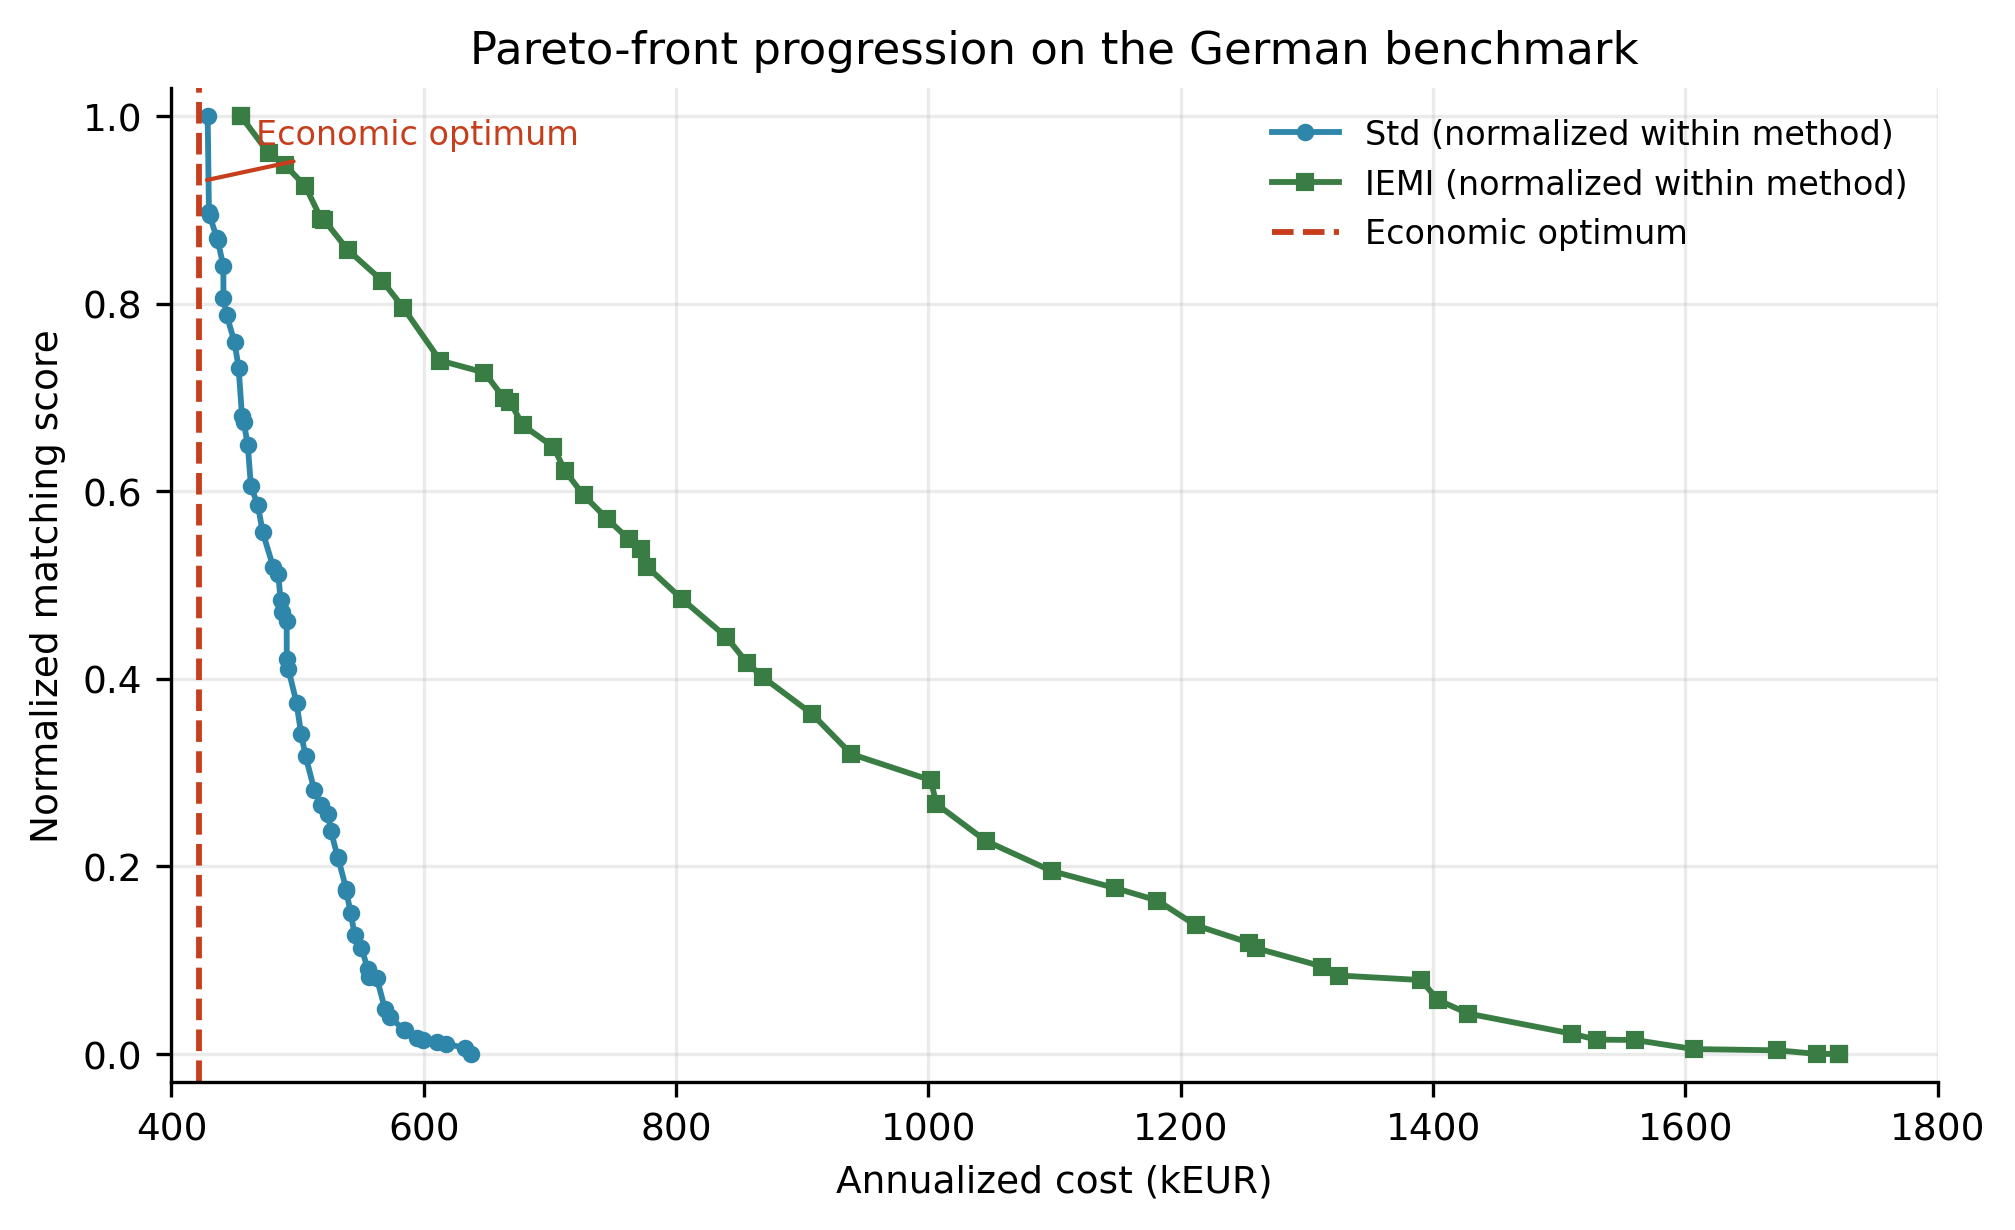
\includegraphics[width=\columnwidth]{figures/pareto_normalized.png}
\caption{Pareto-front progression after within-method normalization of the matching metric. Normalization is used only to visualize front shape and reachable cost span.}
\label{fig:pareto_norm}
\end{figure}

\begin{table}[t]
\centering
\caption{Pareto characteristics, German case ($N_{\text{ind}}{=}50$, $G_{\text{max}}{=}100$).}
\label{tab:conf_pareto}
\small
\begin{tabular}{@{}lccc@{}}
\toprule
& \textbf{A} Economic & \textbf{B} Std & \textbf{C} IEMI \\
\midrule
Pareto points stored & 1 & 50 & 50 \\
Min.\ cost (kEUR) & 422 & 429 & 455 \\
Max.\ cost (kEUR) & --- & 637 & 1{,}722 \\
Front width (kEUR) & --- & 209 & \textbf{1{,}267} \\
Ratio vs.\ Std & --- & $1.0\times$ & \textbf{$6.1\times$} \\
\bottomrule
\end{tabular}
\end{table}

Fig.~\ref{fig:pareto_norm} shows the same fronts after within-method normalization, avoiding the misleading impression that Std and IEMI objective values are directly comparable in magnitude.

\subsection{Budget-aligned operational indicators}
\label{sec:budget}

Selected Pareto points are re-simulated over 8760 hours using the protocol of Section~\ref{sec:case}. Table~\ref{tab:conf_budget} reports the +100\% budget-allowance case. The listed annualized costs are the \emph{actual} costs of the selected designs: Std saturates at EUR~637k, whereas IEMI still offers lower-mismatch alternatives and reaches EUR~869k within the allowed tolerance band.

\begin{table}[t]
\centering
\caption{Operational indicators at +100\% budget, German case (selected Pareto points).}
\label{tab:conf_budget}
\scriptsize
\resizebox{\columnwidth}{!}{%
\begin{tabular}{@{}lcccc@{}}
\toprule
Method & Cost (kEUR) & Peak grid (kW) & Annual grid (MWh) & Self-suff.\ (\%) \\
\midrule
Std  & 637 & 2{,}617 & 15{,}374 & 38.6 \\
IEMI & 869 & \textbf{1{,}920} & \textbf{10{,}781} & \textbf{57.0} \\
\bottomrule
\end{tabular}
}
\end{table}

Relative to Std under the same budget allowance, IEMI reduces peak grid import by 26.7\%, annual grid purchase by 29.9\%, and raises self-sufficiency by 18.3 percentage points. Curtailment remains negligible in both cases, reaching only 0.08\% for the selected IEMI design. The wider IEMI solution set therefore translates into materially different year-round grid interaction.

\begin{figure}[t]
\centering
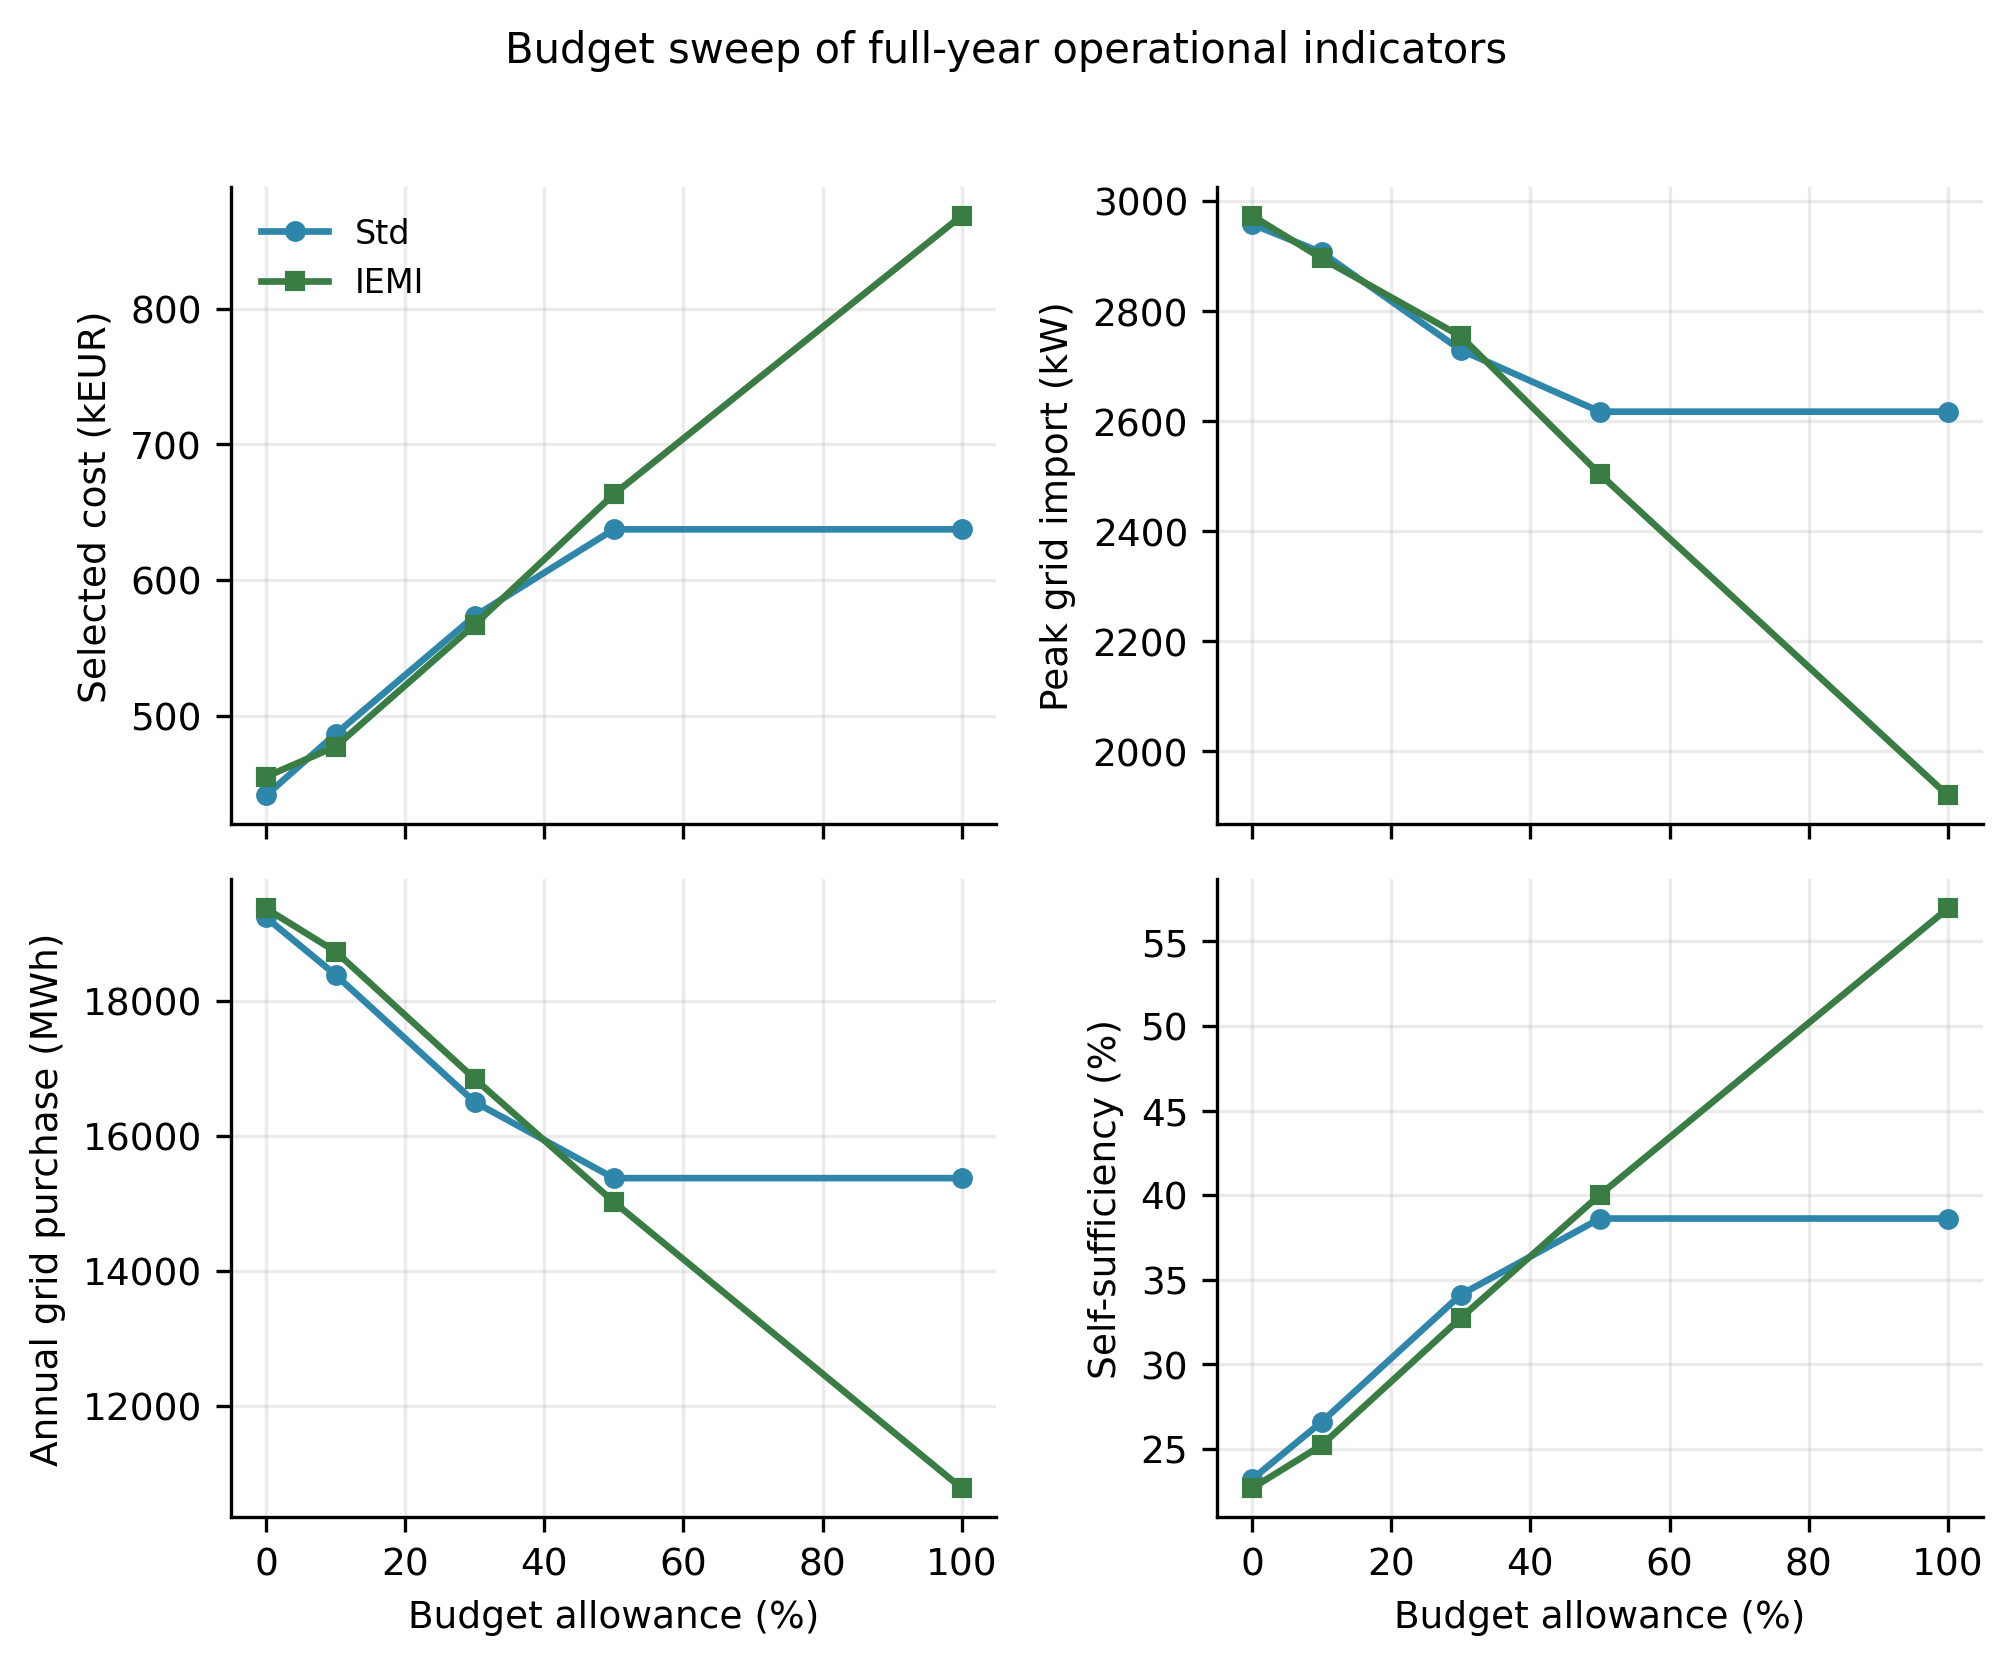
\includegraphics[width=\columnwidth]{figures/budget_sweep.png}
\caption{Full-year operating indicators of budget-aligned designs. Std improves slightly faster under tight budgets, but saturates after +50\%; IEMI overtakes once its wider high-investment region becomes accessible.}
\label{fig:budget_sweep}
\end{figure}

Fig.~\ref{fig:budget_sweep} also shows that IEMI is \emph{not} uniformly superior at every budget level. At +10\% and +30\%, Std still gives slightly lower grid purchase and slightly higher self-sufficiency. The crossover appears around +50\%, after which IEMI dominates the reported grid-interaction indicators. The selected +100\% IEMI design also shifts more strongly toward PV, GT, absorption cooling, and cold storage while largely eliminating electric heat-pump and electric-chiller capacity, which is consistent with its lower electric dependence.

\subsection{Structural interpretation}

Std aggregates per-carrier volatility before cross-carrier coupling and becomes relatively insensitive once those fluctuations are already compressed, so NSGA-II sees little further variation in $f_2$. IEMI preserves hour-by-hour coupling across electricity, heat, and cooling, so designs that reduce \emph{simultaneous} multi-carrier mismatch remain distinguishable as investment increases.

\subsection{Scope and threats to validity}

Three cautions bound the present claim. First, Std and IEMI should not be compared through raw $f_2$ magnitude; we therefore rely on front shape, reachable cost span, and 8760-hour downstream indicators. Second, the German case uses archived benchmark tariffs, so the absolute capacity mix is benchmark-specific. Third, the planning stage uses 14 representative days and one documented evolutionary setting; full-year re-dispatch partly mitigates temporal aggregation bias, but broader evidence across climates, tariffs, and random seeds remains future work.
